\documentclass[tikz]{standalone}
\usepackage[english]{babel}
\usepackage[T1]{fontenc}
\usepackage[default]{droidsans}
\usepackage[LGRgreek]{mathastext}
\begin{document}
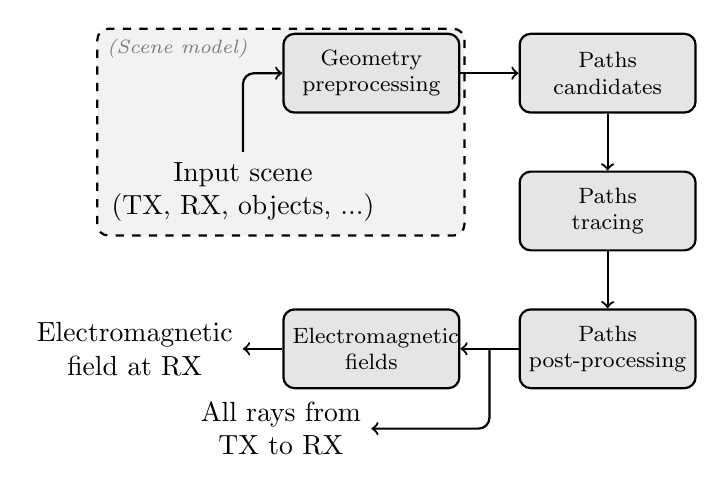
\begin{tikzpicture}[
    node distance=1.0cm and 0.35cm,
    % Styles
    block/.style={
      rectangle,
      draw=black,
      fill=gray!20,
      text width=2.0cm,
      align=center,
      minimum height=1cm,
      rounded corners,
      thick,
      font=\footnotesize,
  }]
  \pgfdeclarelayer{background}
  \pgfsetlayers{background,main}
  \node[block] (gp) at (0,0) {Geometry\\preprocessing};
  \node[block] (pc) at (3.0,0) {Paths\\candidates};
  \node[block] (pt) at (3.0,-1.75) {Paths\\tracing};
  \node[block] (pp) at (3.0,-3.5) {Paths\\post-processing};
  \node[block] (em) at (0,-3.5) {Electromagnetic\\fields};
  \draw[<-,thick, rounded corners] (gp.west) -| ++(-.5,-1) node[below, align=center] (input) {Input scene\\(TX, RX, objects, ...)};
  \draw[->, thick] (gp.east) -- (pc.west);
  \draw[->, thick] (pc.south) -- (pt.north);
  \draw[->, thick] (pt.south) -- (pp.north);
  \draw[->, thick] (pp.west) -- (em.east) node[midway] (midway) {};
  \draw[->, thick, rounded corners] (midway.center) |- ([yshift=-.5cm]em.south) node[left, align=center] {All rays from\\TX to RX};
  \draw[->, thick] (em.west) -- ++(-.5, 0) node[left, align=center] {Electromagnetic\\field at RX};
  \begin{pgfonlayer}{background}
    \draw[thick, rounded corners, dashed, fill=gray!10] ([shift={(+.05,+.05)}]gp.north east) coordinate (A) rectangle ([shift={(-.05,-.05)}]input.south west) coordinate (B);
  \end{pgfonlayer}
  \node[font=\scriptsize,anchor=north west,opacity=0.5] at (B |- A) {\emph{(Scene model)}};
\end{tikzpicture}
\end{document}
